Il presente capitolo illustra le prove sperimentali eseguite per valutare il comportamento dello scheduler. In particolare, si analizza l'assegnazione naive degli ordini al variare del numero di missioni per lotto, confrontando il makespan simulato, il tempo di esecuzione in MATLAB e le ore di lavoro delle singole risorse.

\section{Assegnazione naive delle missioni}
Nell'assegnazione naive, gli ordini vengono selezionati e assegnati alle risorse senza applicare criteri espliciti di bilanciamento del carico o di ottimizzazione. La composizione di ciascun lotto avviene in funzione di una quota prefissata di missioni, rispettando il vincolo di indivisibilità degli ordini.

Si considerano lotti da 20, 40 e 60 missioni. Nei grafici, i marcatori a forma di rombo indicano gli istanti di rifornimento delle risorse; nella prova con 60 missioni per lotto si osservano 19 istanti di rifornimento. Il tempo di esecuzione in MATLAB misura la durata del calcolo, mentre il makespan esprime il tempo di completamento delle attività nel sistema simulato. Le due grandezze devono quindi essere interpretate separatamente.

\subsection{Prova con 20 missioni}
Tra le tre configurazioni considerate, quella con 20 missioni per lotto richiede il maggior numero di richiami dello scheduler. La quota nominale corrisponde a circa due o tre missioni per operatore; l'assegnazione effettiva deve tuttavia rispettare l'indivisibilità degli ordini, che limita la possibilità di ripartire uniformemente il carico.

Le risorse con il maggior numero di ore di lavoro sono la 1, la 4 e la 6. In particolare, la risorsa 4 raggiunge 9.3147 ore, mentre la risorsa 7 presenta il valore minimo, pari a 6.6242 ore. La presenza di ordini di grandi dimensioni, che non possono essere suddivisi tra più risorse, contribuisce allo squilibrio osservato.

La simulazione CTPN persistente richiede 162.962 secondi di esecuzione in MATLAB e presenta un makespan simulato di 9.31 ore. La Figura~\ref{fig:20missionifix} mostra l'andamento della simulazione.

\begin{figure}[htbp]
	\centering
	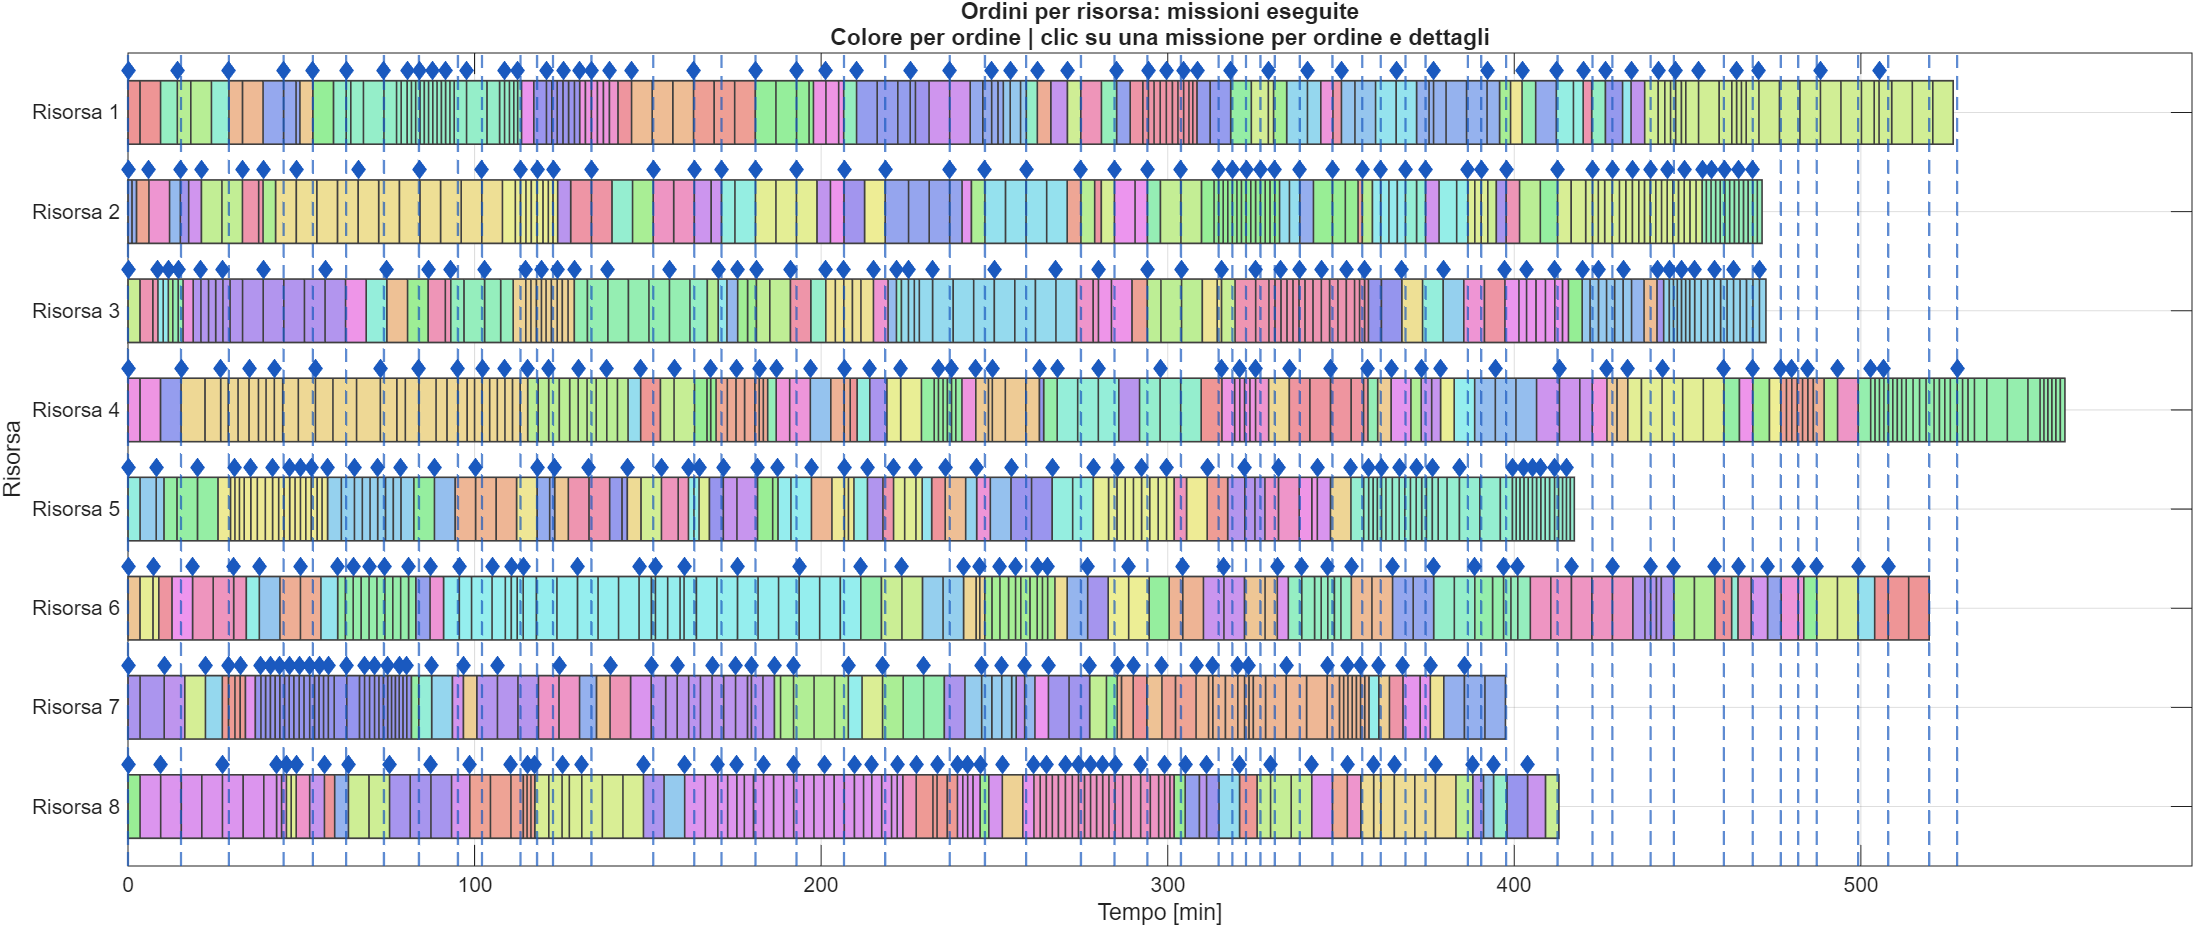
\includegraphics[width=\linewidth]{imgs/esempi/20missioniFIX}
	\caption{Simulazione con assegnazione naive e lotti da 20 missioni.}
	\label{fig:20missionifix}
\end{figure}

\subsection{Prova con 40 missioni}
Con 40 missioni per lotto, il numero di richiami dello scheduler si riduce rispetto alla configurazione precedente. A parità di missioni complessive, il raddoppio della dimensione nominale del lotto comporta indicativamente un dimezzamento del numero di lotti da gestire; il rapporto effettivo dipende dalla composizione degli ordini e dall'eventuale lotto finale incompleto.

Il tempo di esecuzione in MATLAB scende a 156.008 secondi, con una riduzione di circa 6.95 secondi rispetto alla prova con 20 missioni. Questa singola osservazione non consente tuttavia di attribuire la riduzione esclusivamente al minor numero di richiami dello scheduler.

Le ore di lavoro delle risorse diverse dalla 2 sono comprese tra 6.9086 e 8.0386 ore. La risorsa 2 raggiunge invece 9.8656 ore, determinando un makespan simulato di 9.87 ore, superiore a quello della configurazione precedente. Pertanto, la maggiore uniformità osservata per una parte delle risorse non si traduce in una riduzione del tempo complessivo di completamento. La Figura~\ref{fig:40missionifix} riporta la simulazione corrispondente.

\begin{figure}[htbp]
	\centering
	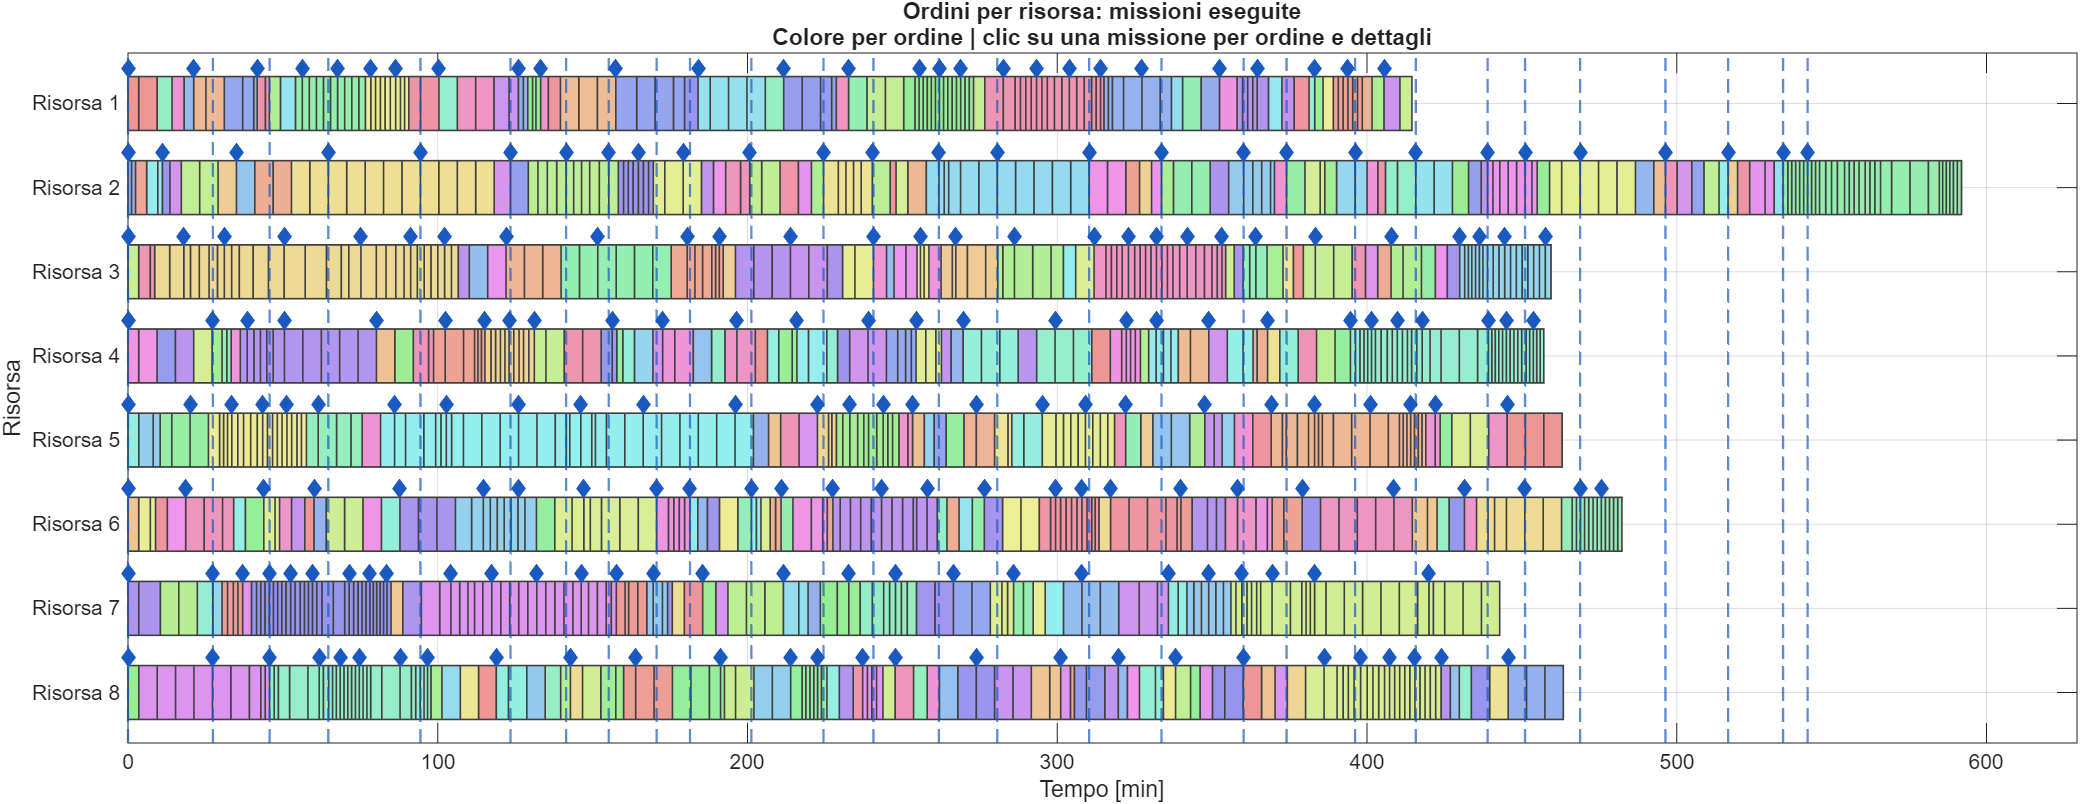
\includegraphics[width=\linewidth]{imgs/esempi/40missioniFIX}
	\caption{Simulazione con assegnazione naive e lotti da 40 missioni.}
	\label{fig:40missionifix}
\end{figure}

\subsection{Prova con 60 missioni}
Con 60 missioni per lotto, il numero nominale di lotti da gestire è circa un terzo rispetto al caso con 20 missioni, a parità di missioni complessive. Anche in questo caso, il numero effettivo di richiami dipende dalla composizione dei lotti.

Il tempo di esecuzione in MATLAB è pari a 156.742 secondi e rimane vicino a quello della prova con 40 missioni. Le ore di lavoro variano da 6.3925 per la risorsa 7 a 9.2633 per la risorsa 4. Il makespan simulato è pari a 9.26 ore, il valore più basso tra le tre prove, sebbene la differenza rispetto al caso con 20 missioni sia contenuta.

L'aumento del numero di missioni per lotto non determina quindi un peggioramento sistematico del makespan. Permane, tuttavia, una distribuzione non uniforme del carico, coerente con l'assenza di un criterio esplicito di bilanciamento nell'assegnazione naive. La Figura~\ref{fig:60missionifix} mostra il risultato della prova.

\begin{figure}[htbp]
	\centering
	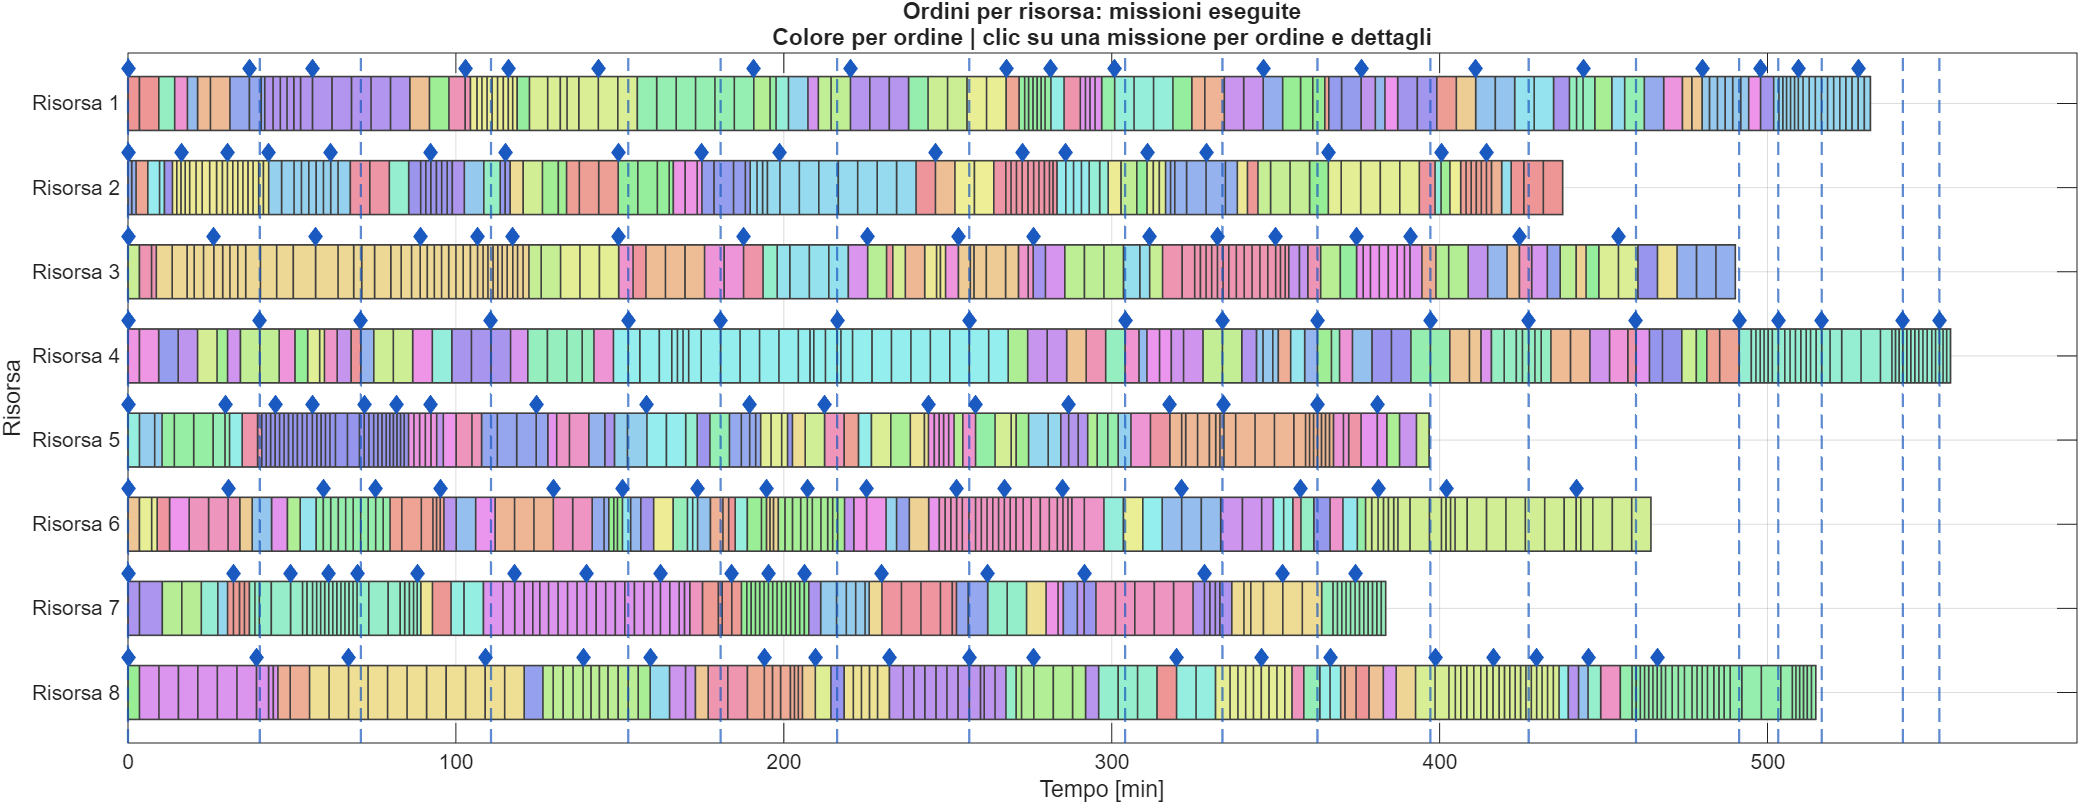
\includegraphics[width=\linewidth]{imgs/esempi/60missioniFIX}
	\caption{Simulazione con assegnazione naive e lotti da 60 missioni.}
	\label{fig:60missionifix}
\end{figure}

\subsection{Confronto dei risultati}
La Tabella~\ref{tab:naive-ore-risorse} riporta le ore di lavoro di ciascuna risorsa nelle tre configurazioni, mentre la Tabella~\ref{tab:naive-riepilogo} sintetizza i tempi di esecuzione e i makespan simulati.

\begin{table}[htbp]
	\centering
	\begin{tabular}{crrr}
		\toprule
		Risorsa & 20 missioni & 40 missioni & 60 missioni \\
		\midrule
		1 & 8.7775 & 6.9086 & 8.8561 \\
		2 & 7.8581 & 9.8656 & 7.2922 \\
		3 & 7.8767 & 7.6569 & 8.1697 \\
		4 & 9.3147 & 7.6181 & 9.2633 \\
		5 & 6.9553 & 7.7167 & 6.6133 \\
		6 & 8.6619 & 8.0386 & 7.7408 \\
		7 & 6.6242 & 7.3806 & 6.3925 \\
		8 & 6.8811 & 7.7231 & 8.5789 \\
		\bottomrule
	\end{tabular}
	
	\caption{Ore di lavoro delle risorse nelle prove con assegnazione naive.}
	\label{tab:naive-ore-risorse}
\end{table}

\begin{table}[htbp]
	\centering
	\caption{Confronto tra tempo di esecuzione in MATLAB e makespan simulato.}
	\label{tab:naive-riepilogo}
	\begin{tabular}{crr}
		\toprule
		Missioni per lotto & Tempo MATLAB (s) & Makespan (h) \\
		\midrule
		20 & 162.962 & 9.31 \\
		40 & 156.008 & 9.87 \\
		60 & 156.742 & 9.26 \\
		\bottomrule
	\end{tabular}
\end{table}

Le differenze tra il massimo e il minimo delle ore di lavoro sono pari a circa 2.69, 2.96 e 2.87 ore, rispettivamente per i lotti da 20, 40 e 60 missioni. Secondo questo indicatore, nessuna delle due configurazioni con lotti più grandi migliora il bilanciamento rispetto alla prova con 20 missioni.

I risultati mostrano che la dimensione del lotto influenza sia la distribuzione del carico sia il makespan, senza evidenziare un andamento monotono. Nelle prove riportate, il lotto da 40 missioni presenta il minor tempo di esecuzione in MATLAB, mentre quello da 60 missioni produce il minor makespan simulato. Queste osservazioni descrivono le esecuzioni considerate e non sono sufficienti, da sole, a stabilire quale dimensione del lotto sia preferibile in generale.
